\documentclass[fontsize=10pt]{article}
\usepackage[utf8]{inputenc}
\usepackage[T1]{fontenc}
\usepackage{graphicx} % handles figures
\usepackage[fleqn]{mathtools}
\usepackage{amsmath}
\usepackage{hyperref}
\usepackage{amssymb}
\usepackage{xcolor}


%%%%%%%%%%%%%%%%
% draw graph ex8
\usepackage{tikz}
\makeatletter
\tikzset{my loop/.style =  {to path={
  \pgfextra{\let\tikztotarget=\tikztostart}
  [looseness=12,min distance=10mm]
  \tikz@to@curve@path},font=\sffamily\small
  }}
\makeatletter
%%%%%%%%%%%%%%%%

%Insertion de tout un tas de librairie qui nous seront probablement inutiles pour la pluspart mais it's always good to have them
\title{\textbf{Maths Discrètes}\\ Solutions TP 4}
\author{Rodrigue Sanchez Lopez}
\date{}
\begin{document}
\maketitle % fais le titre écris plus haut


\section*{Exercice 1}
$(n-1) + (n-2) + (n-3) + \cdots + 1 + 0$

On a n éléments :
\begin{itemize}
    \itemsep0em
    \item Le 1er a une arête vers tous les autres nœuds : $n-1$
    \item Le 2ème a une arête vers tous les autres nœuds sauf le 1er (déjà fait) : $n-2$
    \item Le 3ème a une arête vers tous les autres nœuds sauf les deux précedents (déjà fait) : $n-3$
    \item Etc ...
    \item L'avant dernier a une arête vers le dernier, les autres sont déjà fait : $1$
    \item Le dernier est déjà relié à tous les autres nœuds, il n'y a rien a ajouter : $0$
\end{itemize}

Cela nous donne :

$(n-1) + (n-2) + (n-3) + \cdots + 1 + 0 = \displaystyle\sum_{i=1}^{n-1} i = \frac{n ( n - 1)}{2}$

\section*{Exercice 2}
Rappel du « Handshaking theorem » :
$ \displaystyle\sum_{v \in V} deg(v) = 2 |E|$

En Français : la somme du degré de tous les sommets ($V$) vaut deux fois le nombre de sommet ($E$) (Parce qu'une arête a deux extrémités : elle ajoute $1$ au compte des degrés de chacune de ces extrémitées).

\subsubsection*{Pour $8$ sommets avec chacun $3$ arêtes, nous avons :}
$\displaystyle\sum_{v \in V} dev(v) = 8 * 3 = 24$

$24$ est pair et « marche » donc dans $24 = 2 |E|$ : chaque arête a deux sommet.

\subsubsection*{Pour $7$ et $9$ sommets avec chacun $3$ arêtes, nous avons :}

{\centering $\displaystyle\sum_{v \in V} dev(v) = 7 * 3 = 21$ et $\displaystyle\sum_{v \in V} dev(v) = 9 * 3 = 27$ }

$21$ et $27$ ne sont pas pair et ne respectent donc pas $2 |E|$, dans chacun de ces cas, une des arête n'a pas de « deuxième sommet ».

\section*{Exercice 3}
    Dans un graphe a $n$ sommets, il existe toujours deux nœuds de même degré :

    Soit un graphe $G = (V, E)$ alors : $\exists a, b \in E : deg(a) = deg(b)$

\subsubsection*{Demontrons cela par l'absurde :}
Tous les nœuds ont un degré différent.

Nous avons $n$ nœuds auxquels nous devons attribuer n degrés différents.
La répartition des degrés la plus pertinente est la suivante :

$\{ n - 1, n - 2, \cdots, 0\}$

Notons que un degré plus petit que $0$ ou un degré plus grand que $n - 1$ n'ont pas de sens : On ne peut connaitre un nombre négatif de personne, on ne peut se connaitre soit-même (en plus de tous les autres : degré $n$) et on ne connait pas 2 fois une personne (degré > $n$).

Selon cette répartition, nous avons donc que :
\begin{itemize}
    \itemsep0em
    \item Le premier nœud est donc relié à tous les autres nœuds : $n - 1$\\
        Il connait donc tout le monde.
    \item Le dernier nœud est relié à aucun nœuds : $0$\\
        Il ne connait donc personne.
\end{itemize}
C'est impossible, nous ne pouvons pas avoir dans un même groupe une personne
qui connait tout le monde et en même temps une personne qui ne connait
personne.

Il est donc impossible que tous les nœuds aient des degrés
différents donc au moins deux nœuds ont le même degré.

\section*{Exercice 4}
Nous avons un total de $2n$ nœuds. Démontrons que ce graphe est connexe si le
degré de chaque nœud est plus grand que $n$.

Commençons par diviser nos nœuds en deux sous-ensemble connexe de
$\frac{2n}{2} = n$ nœuds.

Prenons $a$ dans le premier sous-ensemble et $b$
dans le second sous-ensemble.

Dans leurs sous-ensembles respectif, $a$ et $b$
sont relié à tous les autres nœuds ($n-1$), ils ont donc, dans leur sous-ensemble, un
degré de $n - 1$.

Nous avons deux possiblitées :
\begin{description}
    \item [$a$ et $b$ sont adjacent :]
        Ils ont donc un degré de, au moins $(n - 1) + 1 = n$ et le graphe est
        connexe.  \item [$a$ et $b$ ne sont adjacent :] Un degré de $n-1$ ne suffit pas à respecter la condition de l'énoncé.  Ils doivent donc être relié à au moins un nœud de l'autre sous-ensemble
        pour avoir un degré de au moins $n$. Si les deux sous-ensemble sont
        relié, le graphe est connexe.
\end{description}

\section*{Exercice 5}
% récurence sur le nombre d'arêtes

\section*{Exercice 6}
Déterminons le nombre de sommet si
\begin{itemize}
    \item \textbf{G à 12 arêtes et tous les sommets sont de degré 3 :}\\
        Utilisons le « Handshaking theorem » : $ \displaystyle\sum_{v \in V} deg(v) = 2 |E|$\\
        \vspace{-.8em}
        \begin{align*}
            \displaystyle\sum_{v \in V} 3 &= 2 * 12\\
            3 + 3 + (...) + 3 &= 24\\
            |V| * 3 &= 24\\
            |V| &= \frac{24}{3} = 8
        \end{align*}
        Il y a donc $8$ sommets.

    \item \textbf{G à 10 arêtes avec 2 sommets de degré 3 et tous les autres de degré 2 :}\\
        Séparons $V$ en deux sous-ensemble : $V_{1}$ qui contient les deux
        sommets de degré 3 et $V_{2}$ qui contient les autres sommet de degré 2.
        Toujours avec le théorème des poignées de main :
        \vspace{-.8em}
        \begin{align*}
            \displaystyle\sum_{v \in V_{1}} 3 + \displaystyle\sum_{v \in V_{2}} 2 &= 2 * 10\\
            2 * 3 + \displaystyle\sum_{v \in V_{2}} 2 &= 20\\
            \displaystyle\sum_{v \in V_{2}} 2 &= 20 - 6\\
            |V_{2}| * 2 &= 14\\
            |V_{2}| &= \frac{14}{2} = 7
        \end{align*}
        Il y a donc $7$ sommets de degré 3 ($V_{2}$) et 2 sommets de degré
        2 ($V_{1}$). Le total est de 9 sommets.
\end{itemize}

\section*{Exercice 7}
$G$ à $65$ arêtes et $40$ sommets. Chaque sommet est soit de degré $3$ ou $4$.

Pour :\\
$x = \#\text{sommets de degré } 3$\\
$y = \#\text{sommets de degré } 4$\\

Nous avons :\\
$\begin{cases}
    x + y = 40\\
    3x + 4y = 2 * 65 = 130
\end{cases}$\\

Isolons x :
\vspace{-.8em}
\begin{align*}
x = 40 - y\\
\end{align*}
\vspace{-3em}

Calculons y :
\vspace{-.8em}
\begin{align*}
    3(40 - y) + 4y &= 130\\
    120 - 3y + 4y &= 130\\
    -3y + 4y &= 130 - 120\\
    y &= 10
\end{align*}

Et maintenant x :
\vspace{-.8em}
\begin{align*}
x &= 40 - 10\\
x &= 30
\end{align*}

Nous avons donc :
\begin{itemize}
    \itemsep0em
    \item 30 sommets de degré 3
    \item 10 sommets de degré 4
\end{itemize}


\section*{Exercice 8}
\subsection*{Exercice 8.1}

\begin{figure}[!htb]
    \centering
    \begin{minipage}{.7\textwidth}
        Inc = $\begin{bmatrix}
            &(e1)&(e2)&(e3)&(e4)&(e5)&(e6)\\
            (a)&0&0&0&1&0&0\\
            (b)&1&1&0&0&0&1\\
            (c)&0&0&1&0&1&0\\
            (d)&1&0&0&0&0&0\\
            (e)&0&0&1&1&0&0\\
            (f)&0&0&0&0&1&1\\
        \end{bmatrix}$
    \end{minipage}%
    \begin{minipage}{.3\textwidth}
        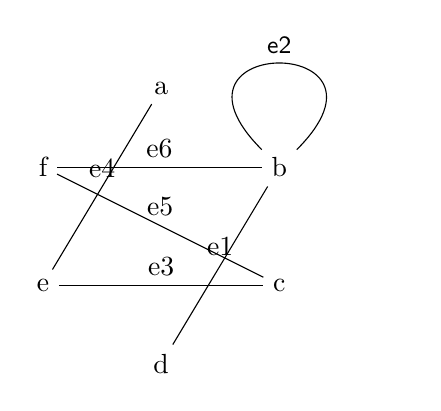
\begin{tikzpicture}
        \path (0,0) node (a) {a}
        (-1.5,-1) node (f) {f}
        (-1.5,-2.5) node (e) {e}
        (1.5,-2.5) node (c) {c}
        (1.5,-1) node (b) {b}
        (0,-3.5) node (d) {d};
        \path
            (b)   edge node[above] {e1}  (d)
            (b)   edge[my loop] node[above] {e2} (b)
            (e)   edge node[above] {e3}  (c)
            (a)   edge node[above] {e4}  (e)
            (f)   edge node[above] {e5}  (c)
            (f)   edge node[above] {e6}  (b);
        \end{tikzpicture}
    \end{minipage}
\end{figure}
Adj = $\begin{bmatrix}
    &(a)&(b)&(c)&(d)&(e)&(f)\\
    (a)&0&0&0&0&1&0\\
    (b)&0&1&0&1&0&1\\
    (c)&0&0&0&0&1&1\\
    (d)&0&1&0&0&0&0\\
    (e)&1&0&1&0&0&0\\
    (f)&0&1&1&0&0&0\\
\end{bmatrix}$

\subsection*{Exercice 8.2}
Ce graphe n'est pas biparti car il possède une boucle sur $b$.

\subsection*{Exercice 8.3}
(cfr théorème 42: slides 93 Chap2F307.pdf ou example 2 dans Revision.pdf)
\par Le nombre de circuit de taille n allant de $v_i$ à $v_j$ est $(i,j)$ dans
$(Adj)^n$.

Commençons par calculer\footnote{Ça n'est que du produit matriciel : \url{https://fr.wikipedia.org/wiki/Produit_matriciel}} $(Adj)^4$ = $\begin{bmatrix}
    2 &1 &3 &0 &0 &0 \\
    1 &12&5 &5 &1 &6 \\
    3 &5 &6 &1 &0 &1 \\
    0 &5 &1 &3 &1 &4 \\
    0 &1 &0 &1 &5 &4 \\
    0 &6 &1 &4 &4 &7 \\
\end{bmatrix}$

Le nombre de circuit de longeur 4 dans $G$ correspond à la somme des valeurs
pour $i = j$, c'est à dire, la diagonal : $2 + 12 + 6 + 3 + 5 + 7 = 35$.

\end{document}
